\documentclass[a4paper,14pt]{extarticle}
\usepackage{../../tex-shared/report-layout}

\renewcommand{\mylabnumber}{1}
\renewcommand{\mylabtitle}{Исследование методов принятия решений в условиях полной неопределенности}
\renewcommand{\mysubject}{Поддержка принятия решений в условиях неопределенности}
\renewcommand{\mylecturer}{Кротов К.В.}

\begin{document}
\begin{titlepage}
    
    \thispagestyle{empty}
    
    \begin{center}
        
        Министерство науки и Высшего образования Российской Федерации \\
        Севастопольский государственный университет \\
        Кафедра ИС
        
        \vfill

        Отчет \\
        по лабораторной работе №\mylabnumber \\
        \enquote{\mylabtitle} \\
        по дисциплине \\
        \enquote{\MakeTextUppercase{\mysubject}}

    \end{center}

    \vspace{1cm}

    \noindent\hspace{7.5cm} Выполнил студент группы ИС/б-17-2-о \\
    \null\hspace{7.5cm} Горбенко К. Н. \\
    \null\hspace{7.5cm} Проверил \\
    \null\hspace{7.5cm} \mylecturer

    \vfill

    \begin{center}
        Севастополь \\
        \the\year{}
    \end{center}

\end{titlepage}

\section{Цель работы}
Изучить и исследовать методы принятия решений при отсутствии какой-либо
информации о связях принимаемых решений и исходов.

\section{Задание на работу}
Для рассмотренной в варианте 2 постановки задачи закупки оборудования в
соответствии с приведенной ниже платежной матрицей, выполнить определение
эффективных решений  с использованием критерия Сэвиджа. Планируется выпуск
новой продукции, для чего необходимо закупить станки. Система оптовой торговли
может поставить не более 50 станков; комплект поставки - 10 станков. Минимальный
объем поставок - 20 станков. Соответственно, вектор решений об объеме поставок X
= (20,30,40,50). Ежегодный доход от продукции, снимаемой с одного станка,
cоставляет 21.9 тыс.руб. Оптовая цена одного станка 4.775 тыс. руб.,
эксплуатационные расходы - 3.6 тыс. руб. Затраты на подготовку производства
составляют 25.5 тыс.руб. и не зависят от числа станков и объема выпуска. Пусть
спрос пропорционален количеству продукции, снимаемой с S работающих станков, и
для простоты ограничимся вектором состояний спроса S = (0,10,20,30,40,50). Если
решающее правило сформулировать как \enquote{доход - издержки}, то можно рассчитать
элементы матрицы полезности: 

$$ W_{ij} = (21.9 - 3.6) * min (x_i, s_j) - 4.775x_i - 25.5 .$$

Тогда вид платежной матрицы следующий:

\begin{table}[H]
    \caption{Платежная матрица}
    \begin{tabular}{ | p{1.9cm} | p{1.9cm} | p{1.9cm} | p{1.9cm} | p{1.9cm} | p{1.9cm} | p{1.9cm} | }
        \hline
         & $S_1=0$ & $S_2=10$ & $S_3=20$ & $S_4=30$ & $S_5=40$ & $S_6=50$ \\ \hline
        $X_1=20$ & 0 & 0 & 0 & -135.25 & -270.5 & -405.75 \\ \hline
        $X_2=30$ & -47.75 & -47.75 & -47.75 & 0 & -135.25 & -270.5 \\ \hline
        $X_3=40$ & -95.5 & -95.5 & -95.5 & -47.75 & 0 & -135.25 \\ \hline
        $X_4=50$ & -143.25 & 143.25 & -143.25 & -95.5 & -47.5 & 0 \\ \hline
    \end{tabular}
\end{table}

\section{Ход работы}
Определение эффективных решений с использованием критерия Сэвиджа:
\begin{table}[H]
    \caption{Платежная матрица}
    \begin{tabular}{ | p{1.4cm} | p{1.4cm} | p{1.4cm} | p{1.4cm} | p{1.4cm} | p{1.4cm} | p{1.4cm} | p{1.4cm} | p{1.4cm} |}
        \hline
         & $S_1=0$ & $S_2=10$ & $S_3=20$ & $S_4=30$ & $S_5=40$ & $S_6=50$ & $f_{ir} = min a_{ij}$ & $min f_{ir} $ \\ \hline
        $X_1=20$ & 0 & 0 & 0 & -135.25 & -270.5 & -405.75 & 405.75 & \\ \hline
        $X_2=30$ & -47.75 & -47.75 & -47.75 & 0 & -135.25 & -270.5 & 270.5 & \\ \hline
        $X_3=40$ & -95.5 & -95.5 & -95.5 & -47.75 & 0 & -135.25 & 135.25 & 135.25 \\ \hline
        $X_4=50$ & -143.25 & 143.25 & -143.25 & -95.5 & -47.5 & 0 & 145.25 & \\ \hline
    \end{tabular}
\end{table}

Текст программы:
\begin{lstlisting}
int main(int argc, char** argv) 
{	setlocale(LC_ALL, "RUSSIAN");
    int i,j;
    float **x;
    float *max_stlb;
    FILE *inp;
    ifstream in("D:\\tpr1.txt");
    string s;
    int n = 0;
    int numCollums;
    while (in.peek() != EOF) {
        getline(in, s);
        numCollums =std::count( s.begin(), s.end(), '\t' ) + std::count( s.begin(), s.end(), ' ' ) + 1;
        n++;
    }
    in.seekg(0, ios::beg);
    in.clear();
    x = new float*[n];
    for (i = 0; i<n; i++) x[i] = new float[numCollums];


    if ((inp = fopen("D:\\tpr1.txt", "r")) == NULL)
    {
        cout<< "Error by open" <<endl;
        return -1;
    }
    else
    for (i = 0; i<n; i++)
        for (j = 0; j<numCollums; j++)
            fscanf(inp, "%f", &x[i][j]);

    fclose(inp);
    cout<< "Payment matrix:" <<endl<<endl;
    for (i = 0 ; i<n; i++)
    {   cout<<'X'<<i+1<<"| ";
        for (j = 0; j<numCollums; j++)
            cout<< x[i][j] << " ";
        cout<<endl;
    }
    cout<<endl<<endl;
    
    
    
        float **ost = new float*[n];
        max_stlb = new float[numCollums];
        float *min_str = new float[n];
        
        for (j = 0; j<numCollums; j++) max_stlb[j]=x[0][j];
        for (j = 0; j<n; j++) min_str[j]=x[j][0];
        
        for (j = 0; j<numCollums; j++)
        for (i = 0; i<n; i++) {
            if (x[i][j]>max_stlb[j]) max_stlb[j]=x[i][j];
        }
        for (j = 0; j<numCollums; j++) cout<<max_stlb[j]<<' ';	
    
        for (i = 0; i<n; i++) ost[i] = new float[numCollums];
        for (i = 0; i<n; i++)
        for (j = 0; j<numCollums; j++){
            ost[i][j]=max_stlb[j]-x[i][j];
        }	
    cout<<endl<< "Residual matrix:" <<endl<<endl;
    cout<<endl;
    for (i = 0 ; i<n; i++)
    {   cout<<'X'<<i+1<<"| ";
        for (j = 0; j<numCollums; j++)
            cout<< ost[i][j] << " ";
        cout<<endl;
    }

    cout<<endl<<endl;
                
        for (j = 0; j<n; j++) min_str[j]=ost[j][0];
        
        for (i = 0; i<n; i++)
        for (j = 0; j<numCollums; j++){
            if (ost[i][j]>min_str[i]) min_str[i]=ost[i][j];
        }
    for (j = 0; j<n; j++) cout<<min_str[j]<<' ';
    
    int ans=0;
    float min=min_str[0];
    for (j = 0; j<n; j++) 
        if(min_str[j]<min) {
            min=min_str[j];
            ans=j;}
    cout<<endl<<"Result: X"<<ans+1<<endl;
    
    for (i = 0; i<n; i++) delete[] x[i];
    delete[] x;
    system("pause");
    in.close();
    return 0;
}
\end{lstlisting}

Результат работы программы представлен на рисунке \ref{fig:result}:

\begin{figure}[H]
    \centering
    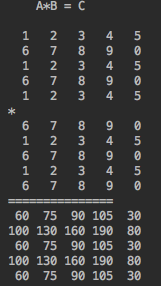
\includegraphics[width=.5\linewidth]{result}
    \caption{Результат работы программы}
    \label{fig:result}
\end{figure}

\section{Вывод}
В ходе выполнения лабораторной работы исследовали применение критерия Сэвиджа
для нахождения эффективных решений в условиях полной неопределенности. Поиск
решений был выполнен как с помощью расчетов вручную, так и с помощью
разработанной программы, результаты поиска решений совпали.
\end{document}